\cleardoublepage                                   
\chapter{Agente de Carga (AC)}

\section{Hardware}
El AC está implementado sobre una placa de desarrollo basada en un microcontrolador ESP32 de 32 bits. La elección de esta plataforma responde a su adecuada capacidad de procesamiento e interfaces para las tareas requeridas, su amplia disponibilidad en el mercado junto a un bajo costo y la extensa base de recursos técnicos existentes, lo que facilita su programación y mantenimiento. Este dispositivo integra las funciones de adquisición de datos, cálculo de variables eléctricas y comunicación tanto con la microrred como con los NC.

El sistema cuenta en primer lugar con una etapa de alimentación encargada de acondicionar la tensión de corriente alterna proveniente de la microrred para energizar el circuito completo. La estabilidad de esta fuente es fundamental, ya que variaciones significativas en su salida introducen errores en las mediciones realizadas por el AC o pueden afectar el desempeño del microcontrolador.

Para la medición de la tensión de la microrred se emplea un módulo sensor basado en el transformador de señal ZMPT101B, seleccionado tanto por sus características técnicas como por su disponibilidad comercial. Este módulo genera una señal sinusoidal con un nivel de continua (offset) y una amplitud proporcional a la tensión real medida. Antes de ser leída por la entrada analógica del microcontrolador, la señal atraviesa una etapa de adecuación que garantiza que sus valores se mantengan dentro del rango permitido por el ESP32, evitando sobrepasar el límite máximo de 3,3 V.

Con el fin de comunicarse con los demás agentes que intervienen en la microrred, el AC incorpora un módulo CAN basado en el controlador MCP2515. Este dispositivo actúa como interfaz física entre el microcontrolador y el bus diferencial del protocolo CAN, permitiendo tanto el envío como la recepción de mensajes. El módulo se conecta al ESP32 mediante la interfaz SPI, a través de la cual se gestionan las señales de control (CS, INT) asociadas a la transmisión y recepción de datos.

El intercambio de información entre el AC y los NC se complementa mediante el protocolo inalámbrico ESP-NOW, soportado nativamente por el ESP32. Este protocolo opera en la banda Wi-Fi pero utiliza directamente la capa de enlace de datos. Al prescindir de redes Wi-Fi existentes, encabezados adicionales y procesos de reensamblado, ofrece baja latencia y alta confiabilidad en enlaces de corto a mediano alcance.

En virtud de la naturaleza distribuida del sistema, el AC también actúa como receptor de los datos de consumo enviados por todos los NC. Estos valores, junto con los parámetros globales de consumo y generación de la microrred que el propio AC calcula, son transmitidos mediante una interfaz UART a un módulo ESP32-S3 Super Mini. Este módulo tiene como función publicar la información recibida en un servidor externo para su almacenamiento, visualización y análisis posterior, permitiendo así integrar la operación local de la microrred con herramientas remotas de supervisión.

Finalmente, el AC incorpora una interfaz local destinada a la interacción con el usuario. Esta incluye un display que proporciona retroalimentación visual inmediata y que se comunica con el microcontrolador mediante la interfaz serie I²C. Se integran además pulsadores que permiten navegar entre distintas pantallas e ingresar parámetros operativos del Sistema de Gestión de Consumo (SGC), facilitando su configuración y supervisión sin necesidad de herramientas externas.

\begin{figure}[hbt!]
    \centering
    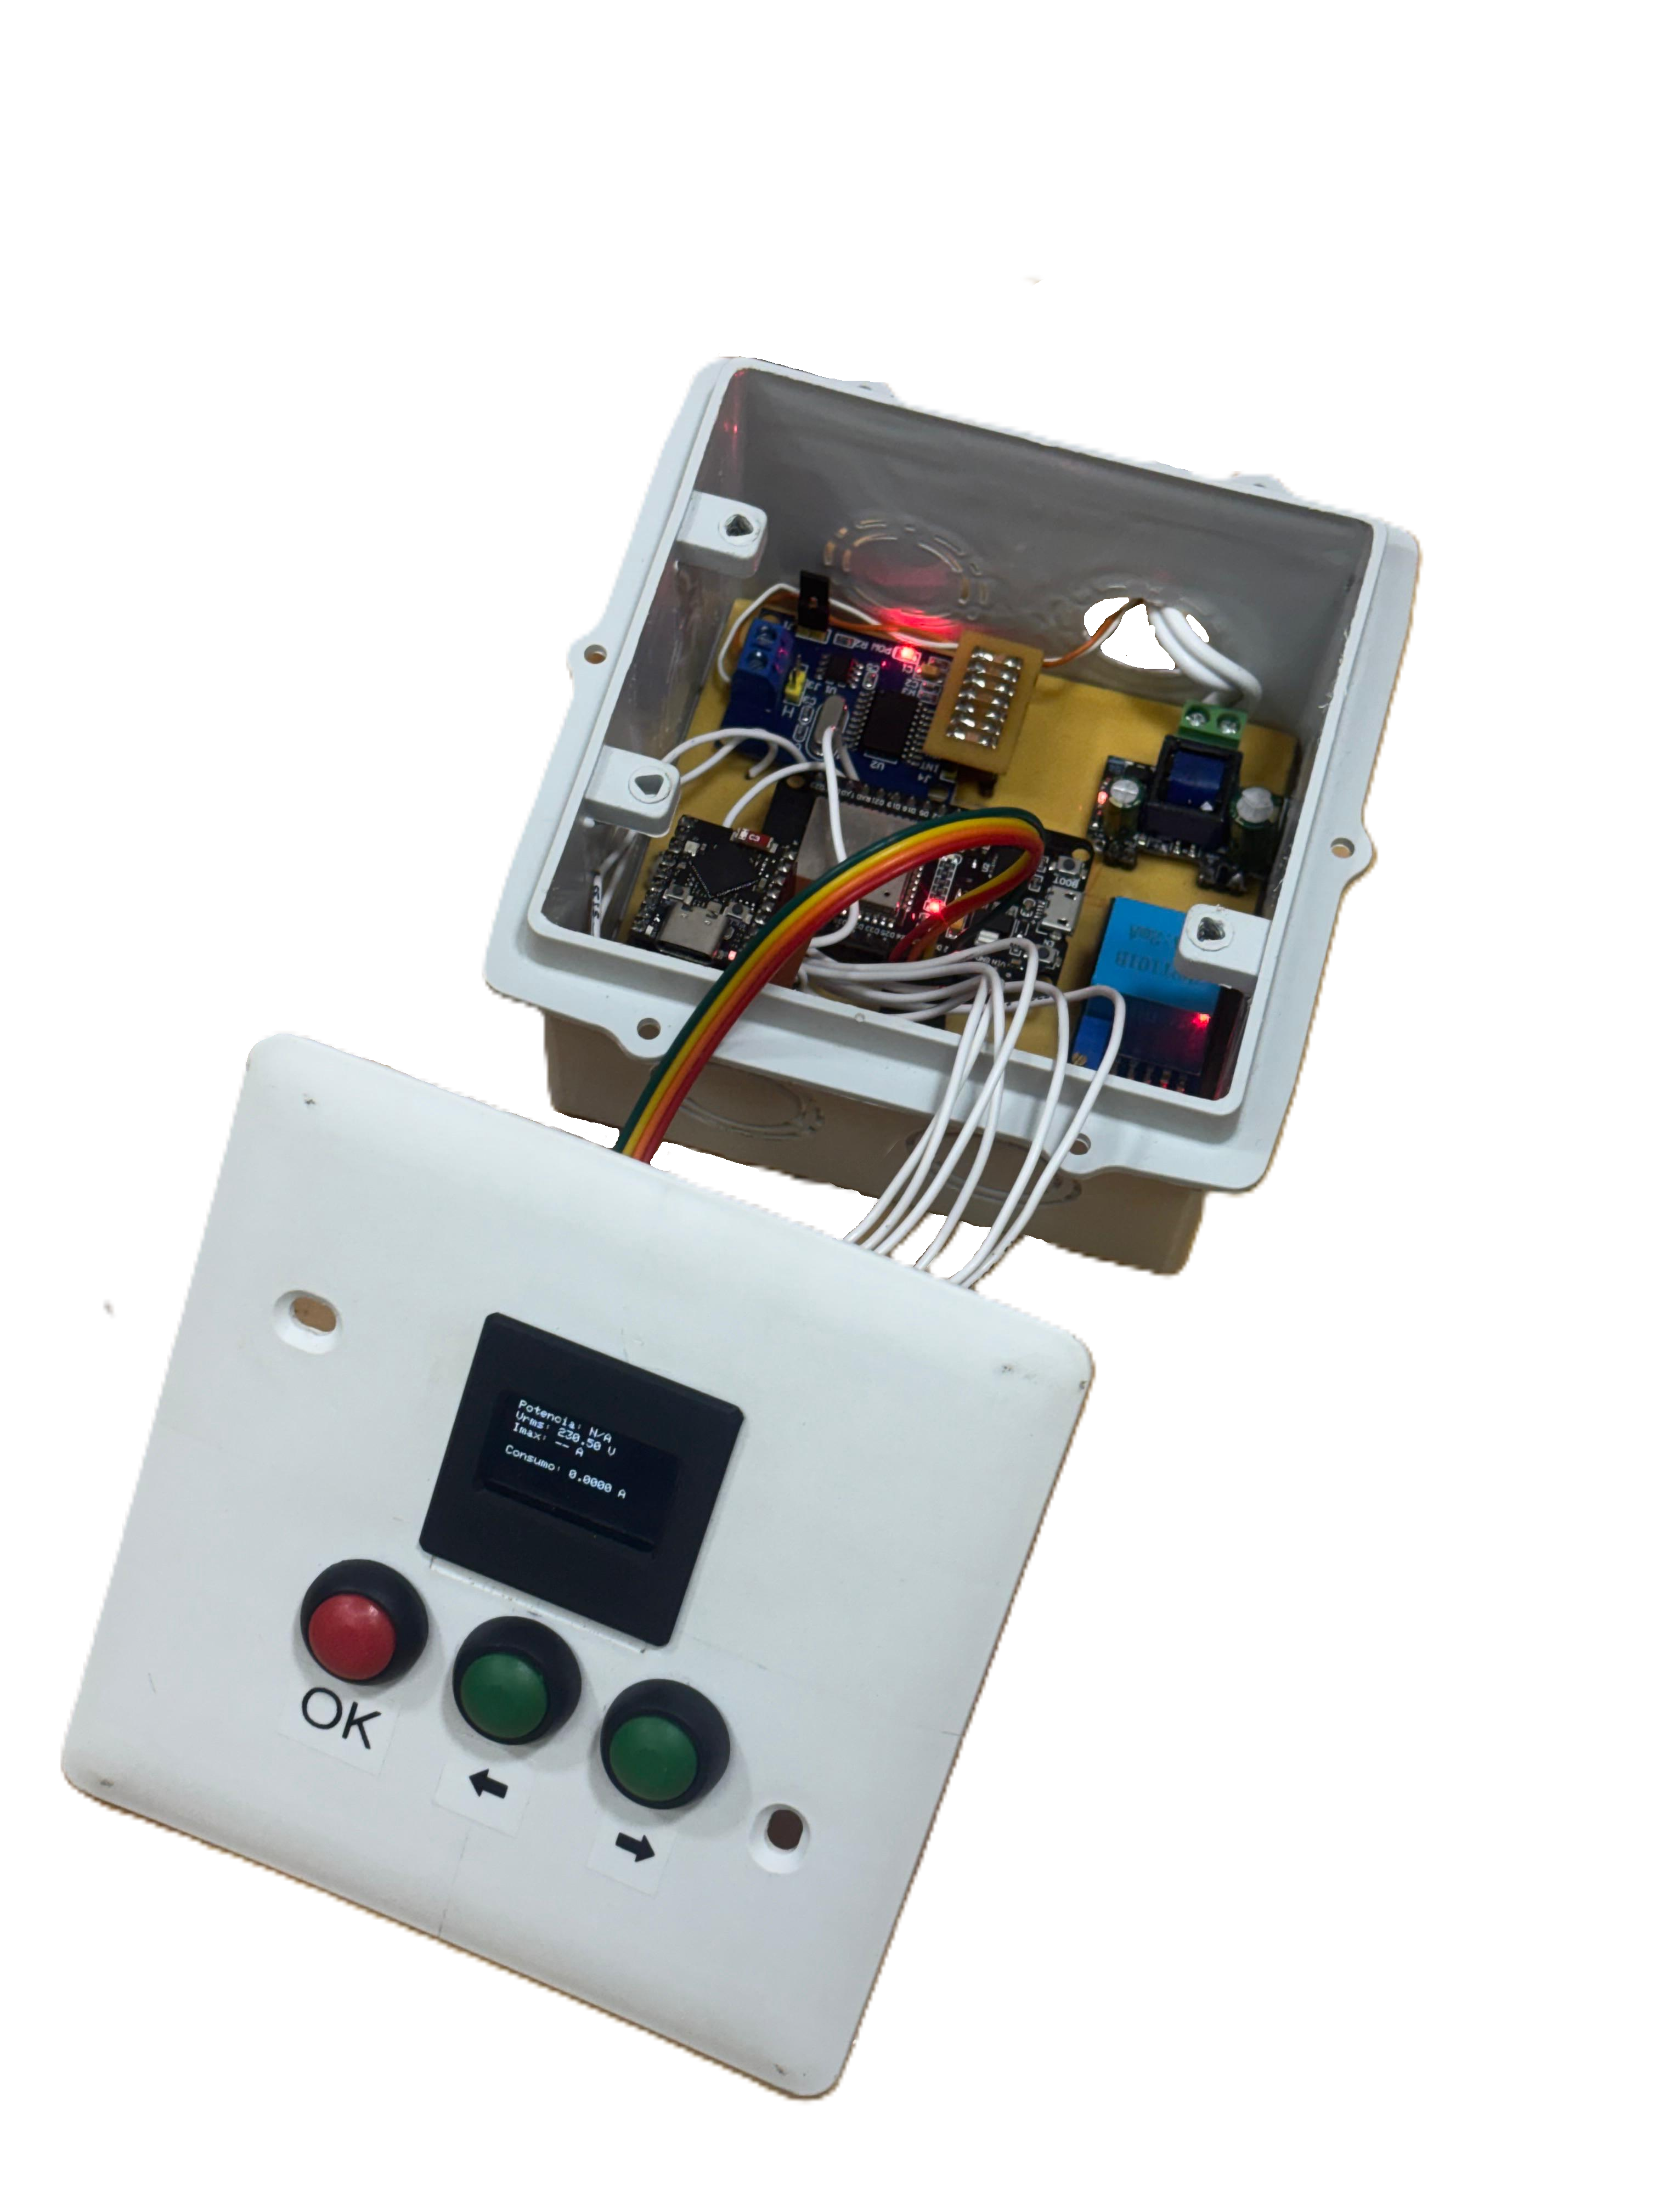
\includegraphics[width=0.35\textwidth]{imagenes/ac.png}
    \caption{Hardware desarrollado para el Agente de Carga(AC)}
    \label{img:ac}
\end{figure}
\section{Firmware}
